% Chapter Template

\chapter{Theory} % Main chapter title

\label{Chapter2} % Change X to a consecutive number; for referencing this chapter elsewhere, use \ref{ChapterX}

%----------------------------------------------------------------------------------------
%	SECTION 1
%----------------------------------------------------------------------------------------

\section{Microwave Resonators}

In most low frequency AC circuits, we are used to transmitting the signal in 2 conductors (or wires). We can do this because at these frequencies, the wavelength of the signal is very large compared to the length of the conductors. In reality, there will be a small phase shift between the signal at the signal generator and the other end of the "wires". This phase shift, along with other phenomena can be easily observed at high frequencies.

At high frequencies, the geometry and properties of the material plays an important role in the transmission. The replacement for what we knew as just "wires" are called \textit{Transmission Lines} or \textit{Waveguides}.

%-----------------------------------
%	SUBSECTION 1
%-----------------------------------
\subsection{Waveguides}

There are many different types of waveguides. Some of them are shown in Fig. \ref{fig:waveguides}. The case we will be dealing with in this thesis pertains to rectangular waveguide.

\begin{figure}
\centering
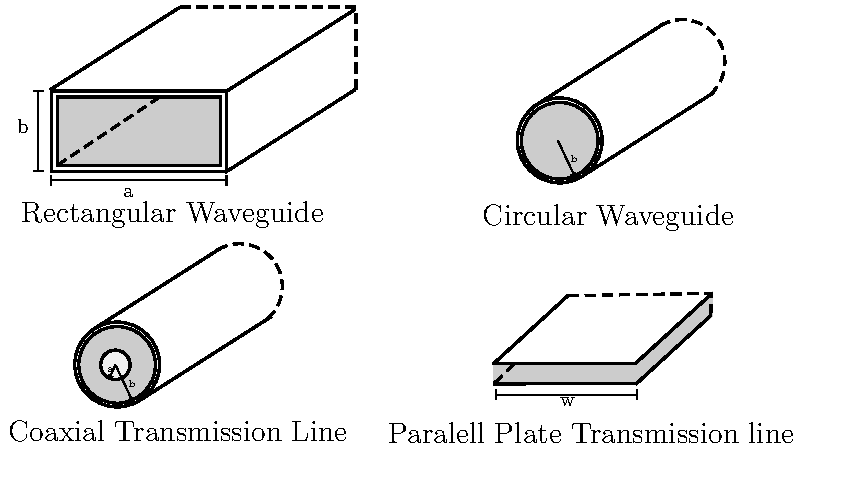
\includegraphics{Figures/Waveguides}
\decoRule
\caption[Waveguide Types]{Types of Waveguides and Transmission Lines}
\label{fig:waveguides}
\end{figure}

\subsubsection{General Waveguide}

Consider a general cross-section of a dielectric surrounded by conductor (can have one more conductor in the dielectric) which continues infinitely along the $z$ axis. We can write down the electric and magnetic fields in the dielectric in phasor domain. We assume that the wave propagates in the $z$-axis and has an $e^{j\omega t}$ dependence.

\begin{equation}
\bar{E}(x,y,z)=[\hat{x}e_x(x,y)+\hat{y}e_y(x,y)+\hat{z}e_z(x,y)]e^{-j\beta z}
\label{eqn:electric field general}
\end{equation}

\begin{equation}
\bar{H}(x,y,z)=[\hat{x}h_x(x,y)+\hat{y}h_y(x,y)+\hat{z}h_z(x,y)]e^{-j\beta z}
\label{eqn:magnetic field general}
\end{equation}

Here $\beta$, the propagation constant, is a real number. $j\beta$ must be replaced with $\gamma=\alpha+j\beta$ if attenuation is also to be considered.

Then, if the dielectric in the waveguide has no charges or currents, we can write Maxwell's equations as

\begin{subequations}
\label{eqn:maxwell curl}
\begin{align}
\nabla \times \bar{E}& =-j\omega \mu \bar{H}
\label{eqn:maxwell electric curl}\\
\nabla \times \bar{H}& =j\omega \epsilon \bar{E}
\label{eqn:maxwell magnetic curl}
\end{align}
\end{subequations}
Taking the curl of \ref{eqn:maxwell electric curl} gives
\begin{equation}
\nabla \times \nabla \times \bar{E}=-j\omega\mu \nabla \times \bar{H}=\omega^2 \mu\epsilon \bar{E}
\end{equation}
Using the vector identity $\nabla\times\nabla\times\bar{A}=\nabla(\nabla .\bar{A})-\nabla^2 \bar{A}$ and $\nabla .\bar{E}=0$ for a region with no sources ($\rho=0$) we get
\begin{equation}
\nabla^2 \bar{E}+\omega^2\mu\epsilon\bar{E}=0
\end{equation}

Similarly, we can also take the curl of \ref{eqn:maxwell magnetic curl} to get
\begin{equation}
\nabla^2 \bar{H}+\omega^2\mu\epsilon\bar{H}=0
\end{equation}

For a $z$ dependence of $e^{-j\beta z}$, $E_z$ and $H_z$ can be written as
\begin{equation}
\left(\frac{\partial^2}{\partial x^2}+\frac{\partial^2}{\partial y^2}+k^2-\beta^2\right)E_z=0
\label{eqn:diff Ez}
\end{equation}
\begin{equation}
\left(\frac{\partial^2}{\partial x^2}+\frac{\partial^2}{\partial y^2}+k^2-\beta^2\right)H_z=0
\label{eqn:diff Hz}
\end{equation}
since $\frac{\partial^2}{\partial z^2}\left(Ae^{-j\beta z}\right)=-\beta Ae^{-j\beta z}$.
Let us define $k_c^2=k^2-\beta^2$ for convenience.

After writing down the 6 equations that arise from \ref{eqn:maxwell curl} and eliminating variables, we can write $E_x$, $E_y$, $H_x$, $H_y$ in terms of $E_z$ and $H_z$ as follows

\begin{subequations}
\label{eqn:general fields}
\begin{align}
E_x& =\frac{-j}{k_c^2}\left(\beta\frac{\partial E_z}{\partial x} + \omega\mu\frac{\partial H_z}{\partial y}\right)
\label{eqn:Ex}
\\
E_y& =\frac{j}{k_c^2}\left(-\beta\frac{\partial E_z}{\partial y}+ \omega\mu\frac{\partial H_z}{\partial x}\right)
\label{eqn:Ey}
\\
H_x& =\frac{j}{k_c^2}\left(\omega\epsilon\frac{\partial E_z}{\partial y}-\beta\frac{\partial H_z}{\partial x}\right)
\label{eqn:Hx}
\\
H_y& =\frac{-j}{k_c^2}\left(\omega\epsilon\frac{\partial E_z}{\partial x}+\beta\frac{\partial H_z}{\partial y}\right)
\label{eqn:Hy}
\end{align}
\end{subequations}
where
\begin{equation}
k_c^2=k^2-\beta^2
\label{eqn:kc definition}
\end{equation}
\begin{equation}
k=\omega \sqrt{\mu\epsilon}=2\pi/\lambda
\label{eqn:k=2pi/lambda}
\end{equation}

These equations (\ref{eqn:diff Ez}, \ref{eqn:diff Hz} and \ref{eqn:general fields}) can be used for any waveguide. There are three types of waves that are possible in waveguides: Transverse Electric and Magnetic mode (TEM), Transverse Electric mode (TE) and Transverse Magnetic mode (TM).

\begin{enumerate}
\item \textbf{TEM modes}

In this mode $E_z=H_z=0$, meaning there are only transverse fields.
\item \textbf{TE modes}

In this mode $E_z=0$, meaning there are only transverse electric fields.
\item \textbf{TM modes}

In this mode $H_z=0$, meaning there are only transverse magnetic fields.
\end{enumerate}

\subsubsection{Rectangular Waveguide}

Let us now concentrate on the fields in a rectangular waveguide. It can be shown that in the TEM mode, fields in the dielectric follow the same rules as electrostatics \cite{Pozar2009}. In a single conductor waveguide like the rectangular waveguide, the electrostatic potential is zero (or constant) which means that $E=0$ and $H=0$. This means we can only have TE and TM modes in the rectangular waveguide (or any single conductor waveguide).

\begin{enumerate}
\item \textbf{TE modes}

Equation \ref{eqn:diff Hz} has been rewritten below with $k^2-\beta^2$ replaced with $k_c$ and divided by $e^{-j\beta z}$.
\begin{equation}
\left(\frac{\partial^2}{\partial x^2}+\frac{\partial^2}{\partial y^2}+k_c^2\right)h_z=0
\label{eqn:hz diff}
\end{equation}
Here, $H_z(x,y,z)=h_z(x,y)e^{-j\beta z}$.

We can solve \ref{eqn:hz diff} using separation of variables. We assume
\begin{equation}
h_z(x,y)=F(x)G(y)
\end{equation}
Substituting this into \ref{eqn:hz diff} gives
\begin{equation}
\frac{1}{F}\frac{d^2F}{dx^2}+\frac{1}{G}\frac{d^2G}{dy^2}+k_c^2=0
\end{equation}
Now, since each term is independent of each other, each term must be a constant. We define the first term to be $k_x^2$ and the second term to be $k_y^2$ to get 
\begin{equation}
k_x^2+k_y^2+k_c^2=0
\end{equation}
Then we get 2 ordinary differential equations
\begin{subequations}
\label{eqn:separation}
\begin{align}
\frac{d^2F}{dx^2}+k_xF& =0\\
\frac{d^2G}{dy^2}+k_yG& =0
\end{align}
\end{subequations}
The general solution to \ref{eqn:separation} is
\begin{subequations}
\begin{align}
F& =A\cos(k_xx)+B\sin(k_xx)\\
G& =C\cos(k_yy)+D\sin(k_yy)
\end{align}
\end{subequations}
Which gives
\begin{equation}
h_z =(A\cos(k_xx)+B\sin(k_xx))(C\cos(k_yy)+D\sin(k_yy))
\label{eqn:hz general}
\end{equation}

Since the boundary conditions we have are that the tangential electric field at the conductor is zero, i.e.
\begin{subequations}
\begin{align}
e_x(x,y)& =0 & \text{ at } y=0 \text{ and } y=b
\label{eqn:ex boundary}\\
e_y(x,y)& =0 & \text{ at } x=0 \text{ and } x=a
\label{eqn:ey boundary}
\end{align}
\end{subequations}

Substituting $E_z=0$ in \ref{eqn:general fields}, we get
\begin{subequations}
\label{eqn:TE transverse diff}
\begin{align}
E_x& =\frac{-j\omega\mu}{k_c^2}\frac{\partial H_z}{\partial y}\\
E_y& =\frac{-j\omega\mu}{k_c^2}\frac{\partial H_z}{\partial x}\\
H_x& =\frac{-j\beta}{k_c^2}\frac{\partial H_z}{\partial x}\\
H_y& =\frac{-j\beta}{k_c^2}\frac{\partial H_z}{\partial y}
\end{align}
\end{subequations}

Now substituting $h_z(x,y)$ from \ref{eqn:hz general} we get the following electric fields
\begin{subequations}
\begin{align}
e_x& =\frac{-j\omega\mu}{k_c^2}k_y(A\cos(k_xx)+B\sin(k_xx))(-C\sin(k_yy)+D\cos(k_yy))\\
e_y& =\frac{j\omega\mu}{k_c^2}k_x(-A\sin(k_xx)+B\cos(k_xx))(C\cos(k_yy)+D\sin(k_yy))
\end{align}
\end{subequations}
Now applying the boundary conditions,\\
from \ref{eqn:ex boundary} we get $D=0$ and $k_y=n\pi/b$ for $n={0,1,2\ldots}$,\\
and from \ref{eqn:ey boundary} we get $B=0$ and $k_x=m\pi/a$ for $m={0,1,2\ldots}$.\\
From this we know the propagation constant is
\begin{equation}
\beta = \sqrt{k^2-k_c^2}=\sqrt{k^2-\left(\frac{m\pi}{a}\right)^2-\left(\frac{n\pi}{b}\right)^2}
\end{equation}
Since $\beta$ is real, we now have a cut-off frequency for which $k^2>k_c^2$. This means that if $a>b$, there will be a range of frequencies for which $TE_{mn}=TE_{10}$ will have propagation but $TE_{01}$ will not.

The final solution for $H_z$ is
\begin{equation}
H_z(x,y,z)=A_{mn}\cos\left(\frac{m\pi x}{a}\right)\cos\left(\frac{n\pi y}{b}\right)e^{-j\beta z}
\label{Hz final}
\end{equation}
where $A_{mn}=AC$.

Now we can find $E_x, E_y, H_x$ and $H_y$ using \ref{eqn:TE transverse diff}
\begin{subequations}
\label{eqn:TE transverse fields}
\begin{align}
E_x(x,y,z)& =\frac{j\omega\mu n\pi}{k_c^2b}A_{mn}\cos\left(\frac{m\pi x}{a}\right)\sin\left(\frac{n\pi y}{b}\right)e^{-j\beta z}\\
E_y(x,y,z)& =\frac{-j\omega\mu m\pi}{k_c^2a}A_{mn}\sin\left(\frac{m\pi x}{a}\right)\cos\left(\frac{n\pi y}{b}\right)e^{-j\beta z}\\
H_x(x,y,z)& =\frac{j\beta m\pi}{k_c^2a}A_{mn}\sin\left(\frac{m\pi x}{a}\right)\cos\left(\frac{n\pi y}{b}\right)e^{-j\beta z}\\
H_y(x,y,z)& =\frac{j\beta n\pi}{k_c^2b}A_{mn}\cos\left(\frac{m\pi x}{a}\right)\sin\left(\frac{n\pi y}{b}\right)e^{-j\beta z}
\end{align}
\end{subequations}

These equations are only for a wave propagating in one direction. The total electric field well have another term for the fields with a different constant. We can replace $A_{mn}$ with $A_{mn}^+$ (for $+z$ direction propagation) and $A_{mn}^-$ (for $-z$ direction propagation). Then the transverse fields for each mode ($m,n$) would take the form
\begin{subequations}
\begin{align}
\bar{E}_t(x,y,z)& =[\hat{x}e_x(x,y)+\hat{y}e_y(x,y)](A^+e^{-j\beta z}+A^-e^{+j\beta z})\\
\bar{H}_t(x,y,z)& =[\hat{x}h_x(x,y)+\hat{y}h_y(x,y)](A^+e^{-j\beta z}-A^-e^{+j\beta z})
\end{align}
\end{subequations}
The negative sign for $A^-$ in the magnetic field is to ensure that the direction of propagation given by $\bar{E}_t\times\bar{H}_t$ is opposite.

\item \textbf{TM modes}

The TM modes can be derived in exactly the same way except that the boundary conditions will apply directly to $E_z$ this time.

The fields for the TM modes are
\begin{subequations}
\begin{align}
E_z(x,y,z)& =B_{mn}\sin\left(\frac{m\pi x}{a}\right)\sin\left(\frac{n\pi y}{b}\right)e^{-j\beta z}\\
E_x(x,y,z)& =\frac{-j\beta m\pi}{k_c^2a}B_{mn}\cos\left(\frac{m\pi x}{a}\right)\sin\left(\frac{n\pi y}{b}\right)e^{-j\beta z}\\
E_y(x,y,z)& =\frac{-j\beta n\pi}{k_c^2b}B_{mn}\sin\left(\frac{m\pi x}{a}\right)\cos\left(\frac{n\pi y}{b}\right)e^{-j\beta z}\\
H_x(x,y,z)& =\frac{j\omega\epsilon n\pi}{k_c^2b}B_{mn}\sin\left(\frac{m\pi x}{a}\right)\cos\left(\frac{n\pi y}{b}\right)e^{-j\beta z}\\
H_y(x,y,z)& =\frac{-j\omega
\epsilon m\pi}{k_c^2a}B_{mn}\cos\left(\frac{m\pi x}{a}\right)\sin\left(\frac{n\pi y}{b}\right)e^{-j\beta z}
\end{align}
\end{subequations}

Notice that if $m$ or $n$ is zero, then the fields all go to zero. So there is no $TM_{10}$ or $TM_{01}$ mode.

The propagation constant $\beta$ is
\begin{equation}
\beta = \sqrt{k^2-k_c^2}=\sqrt{k^2-\left(\frac{m\pi}{a}\right)^2-\left(\frac{n\pi}{b}\right)^2}
\end{equation}

This means the cut-off frequencies are the same for the TE and TM modes. Now we can see that there is a range of frequencies where only the $TE_{10}$ mode will propagate. This feature of waveguides is used extensively to avoid complications of other modes interfering with the signal.
\end{enumerate}


%-----------------------------------
%	SUBSECTION 2
%-----------------------------------

\subsection{Rectangular Waveguide Resonators}

Now that we know what modes and what frequencies can propagate in a rectangular waveguide, we can convert the waveguide into a resonator by walling the 2 infinitely open faces with conducting surfaces to make a cuboid filled with dielectric. This structure is often called a rectangular cavity.\\

We can use the equations we derived in the previous section for fields and the propagation constant to see what effects the new conducting walls will have.

We can start by writing down the transverse electric field ($E_t = \hat{x}E_x+\hat{y}E_y$)
\begin{equation}
\bar{E}_t=\bar{e}(x,y)(A^+e^{-j\beta z}+A^-e^{+j\beta z})
\label{eqn:Et start}
\end{equation}
where $\bar{e}(x,y)$ is the variation in the transverse fields.
\begin{equation}
\beta = \sqrt{k^2-\left(\frac{m \pi}{a}\right)^2-\left(\frac{n \pi}{b}\right)^2}
\end{equation}

The new boundary conditions added now are that $E_t=0$ at the 2 new walls, $z=0$ and $z=d$.\\
Putting $z=0$ into \ref{eqn:Et start} gives 
\begin{equation}
A^+=-A^-
\end{equation}.\\
Putting $z=d$ into \ref{eqn:Et start} gives
\begin{equation}
-\bar{e}(x,y)A^+2j\sin(\beta_{mn}d)=0
\end{equation}
The solution to this equation (other than $A^+=0$) is
\begin{equation}
\beta_{mn}=\frac{l\pi}{d} \text{ where } l=1,2,3\ldots
\end{equation}
This means that, given a frequency, propagation (or in this case resonance) occurs only for particular lengths. $\beta^2=k^2-k_c^2$ can be rearranged to get
\begin{equation}
k_{mnl}=\sqrt{\left(\frac{m \pi}{a}\right)^2+\left(\frac{n \pi}{b}\right)^2+\left(\frac{l \pi}{d}\right)^2}
\end{equation}
The resonant frequency is given by
\begin{equation}
f_{mnl}=\frac{ck_{mnl}}{2\pi\sqrt{\mu_r\epsilon_r}}=\frac{c}{2\pi\sqrt{\mu_r\epsilon_r}}\sqrt{\left(\frac{m \pi}{a}\right)^2+\left(\frac{n \pi}{b}\right)^2+\left(\frac{l \pi}{d}\right)^2}
\end{equation}

Now let us restrict ourselves to the $TE_{10l}$ mode of the resonator. Since $A^-=-A^+$, the fields for this mode are
\begin{subequations}
\label{eqn:TE10l fields}
\begin{align}
E_y(x,y,z)& =A^+\sin\left(\frac{\pi x}{a}\right)(e^{-j\beta z}-e^{+j\beta z})\\
H_x(x,y,z)& =\frac{-A^+}{Z_{TE}}\sin\left(\frac{\pi x}{a}\right)(e^{-j\beta z}+e^{+j\beta z})\\
H_z(x,y,z)& =\frac{j\pi A^+}{k\eta a}\cos\left(\frac{\pi x}{a}\right)(e^{-j\beta z}-e^{+j\beta z})
\end{align}
\end{subequations}
where
\begin{subequations}
\begin{align*}
A^+& =\frac{-j\omega\mu m\pi}{k_c^2a}\\
Z_{TE}& =\frac{\omega\mu}{\beta}& 
k& =\omega\sqrt{\mu\epsilon}\\
k_c^2& =\sqrt{\frac{\pi}{a}}& 
\eta& =\sqrt{\frac{\mu}{\epsilon}}
\end{align*}
\end{subequations}

Using $-2jA^+=E_0$, we can simplify the above equations to
\begin{subequations}
\begin{align}
E_y(x,y,z)& =E_0\sin\left(\frac{\pi x}{a}\right)\sin\left(\frac{l\pi z}{d}\right)\\
H_x(x,y,z)& =\frac{-jE_0}{Z_{TE}}\sin\left(\frac{\pi x}{a}\right)\cos\left(\frac{l\pi z}{d}\right)\\
H_z(x,y,z)& =\frac{j\pi E_0}{k\eta a}\cos\left(\frac{\pi x}{a}\right)\sin\left(\frac{l\pi z}{d}\right)
\end{align}
\end{subequations}

We can now calculate the \textit{quality factor} $Q$ by calculating the energy stored and power lost in the resonator.
The stored electric energy is, from \cite{Pozar2009}
\begin{equation}
W_e=\frac{\epsilon}{4}\int_V E_yE_y^*dv = \frac{\epsilon abd}{16}E_0^2
\end{equation}
and the stored magnetic energy is
\begin{align}
\begin{split}
W_m&=\frac{\mu}{4}\int_V (H_xH_x^*+H_zH_z^*)dv\\
&= \frac{\mu abd}{16}E_0^2\left(\frac{1}{Z_{TE}^2}+\frac{\pi^2}{k^2\eta^2a^2}\right)\\
&=\frac{\mu abd}{16}E_0^2\left(\frac{\beta^2+(\pi/a)^2}{k^2\eta^2}\right)\\
&=\frac{\mu abd}{16}E_0^2\left(\frac{1}{\eta^2}\right)\\
&=\frac{\epsilon abd}{16}E_0^2
\end{split}
\end{align}
Note that $W_e=W_m$ at resonance.

The power lost by the conducting walls is
\begin{equation}
P_c=\frac{R_s}{2}\int_{walls} |H_t|^2ds
\end{equation}
where $R_s=\sqrt{\omega\mu_0/w\sigma}$ is the surface resistivity and $H_t$ is the tangential magnetic field at the walls. This gives
\begin{equation}
P_c=\frac{R_sE_0^2\lambda^2}{8\eta^2}\left(\frac{l^2ab}{d^2}+\frac{bd}{a^2}+\frac{l^2a}{2d}+\frac{d}{2a}\right)
\end{equation}

The power dissipated from the lossy dielectric with $\epsilon = \epsilon'-j\epsilon''$ is
\begin{equation}
P_d = \frac{1}{2}\int_V\bar{J}.\bar{E}=\frac{\omega\epsilon''}{2}\int_V|\bar{E}|^2dv=\frac{abd\omega\epsilon''|E_0|^2}{8}
\end{equation}

The quality factor $Q$ is defined as
\begin{align}
\begin{split}
Q&=\omega\frac{\text{average energy stored}}{\text{average power loss}}\\
&=\omega\frac{W_e+W_m}{P_{loss}}\\
&=\omega\frac{2W_e}{P_c+P_d}
\end{split}
\end{align}

\subsection{Coupling to an External Circuit}

\iffalse
A resonator is useless if we cannot communicate with it in some way. There are many ways of interacting with a resonator. In the experiments to follow, the rectangular cavity resonator will be coupled to and external circuit through a probe of height $h$ inserted at the $y=0$ wall at $x=a/2$ and $z=z_0$. A figure of the probe inserted in the rectangular cavity is shown in Fig.\ref{fig:Probe}.

%---------FILL THE PROBE FIGURE------------------------

To determine the amplitude of the wave generated due to a current density $\bar{J}(x,y,z)$ in the resonator, we can use the reciprocity theorem derived in \cite{Pozar2009}.
\begin{equation}
\label{eqn:reciprocity Th}
\oint_S \left( \bar{E}_1 \times\bar{H}_2 - \bar{E}_2 \times\bar{H}_1\right)\cdot d\bar{s}=\int_V \left(\bar{E}_2\cdot\bar{J}_1 - \bar{E}_1\cdot\bar{J}_2\right)dv
\end{equation}

Let us separate the left moving wave and right moving wave of the $TE_{101}$ mode from \ref{eqn:TE10l fields} in order to use the theorem.
\begin{subequations}
\begin{align}
\bar{E}^+&=-A^+\sin\left(\dfrac{\pi x}{a}\right)e^{(j\pi z/d)} \hat{y}\\
\bar{E}^-&=A^+\sin\left(\dfrac{\pi x}{a}\right)e^{-(j\pi z/d)} \hat{y}\\
\bar{H}^+&=-\dfrac{A^+}{Z_{TE}}\sin\left(\dfrac{\pi x}{a}\right)e^{(j\pi z/d)} \hat{x}-\dfrac{j\pi A^+}{k\eta a}\cos\dfrac{\pi x}{a}e^{(j\pi z/d)} \hat{z}\\
\bar{H}^-&=-\dfrac{A^+}{Z_{TE}}\sin\left(\dfrac{\pi x}{a}\right)e^{-(j\pi z/d)} \hat{x}+\dfrac{j\pi A^+}{k\eta a}\cos\dfrac{\pi x}{a}e^{(-j\pi z/d)} \hat{z}\\
\end{align}
\end{subequations}
Now let
\begin{align}
\bar{E}_1&=\bar{E}^++\bar{E}^-&&\bar{E}_2=\bar{E}^-\\
\bar{H}_1&=\bar{H}^++\bar{H}^-&&\bar{H}_2=\bar{H}^-\\
\bar{J}_1&=\bar{J}&&\bar{J}_2=0
\end{align}
Now $\bar{E}_1,\bar{H}_1$ (which are the $TE_{101}$ fields) are generated by the current in the probe ($\bar{J}_1$) and $\bar{E}_2,\bar{H}_2$ do not have any source.

Using the reciprocity theorem,
\begin{align}
\begin{split}
\label{eqn:lhs reciprocity}
LHS&=\oint_S \left( \bar{E}_1 \times\bar{H}_2 - \bar{E}_2 \times\bar{H}_1\right)\cdot d\bar{s}\\
&= \oint_S \left( (\bar{E}^+ \times\bar{H}^-) +(\bar{E}^- \times\bar{H}^-) - (\bar{E}^- \times\bar{H}^+)-(\bar{E}^- \times\bar{H}^-)\right)\cdot d\bar{s}\\
&=\oint_S \left( (\bar{E}^+ \times\bar{H}^-) - (\bar{E}^- \times\bar{H}^+)\right)\cdot d\bar{s}\\
&=\oint_S\biggl[ \left\lbrace-\dfrac{(A^+)^2}{Z_{TE}}\sin^2\left(\dfrac{\pi x}{a}\right)(+\hat{z})-\dfrac{j\pi (A^+)^2}{k\eta a}\sin\left(\dfrac{\pi x}{a}\right)\cos\left(\dfrac{\pi x}{a}\right)(+\hat{x})\right\rbrace\\
&\quad-\left\lbrace\dfrac{(A^+)^2}{Z_{TE}}\sin^2\left(\dfrac{\pi x}{a}\right)(+\hat{z})+\dfrac{j\pi (A^+)^2}{k\eta a}\sin\left(\dfrac{\pi x}{a}\right)\cos\left(\dfrac{\pi x}{a}\right)(+\hat{x})\right\rbrace\biggr]\cdot d\bar{s}\\
&=2\oint_S \left[-\dfrac{(A^+)^2}{Z_{TE}}\sin^2\left(\dfrac{\pi x}{a}\right)(+\hat{z})-\dfrac{j\pi (A^+)^2}{k\eta a}\sin\left(\dfrac{\pi x}{a}\right)\cos\left(\dfrac{\pi x}{a}\right)(+\hat{x})\right]\cdot d\bar{s}
\end{split}
\end{align}
Where $V$ is any finite volume that surrounds the probe (or current source) and $S$ is the closed surface enclosing it. Let us choose $S$ as the cuboid formed by the $z=z_1$ and $z=z_2$ planes ($0<z_1<z_0$ and $z_0<z_2<d$) and the $x=0,a$ and $y=0,b$ planes which are the walls of the resonator.

Since there is no $y$ component in the integrand of \ref{eqn:lhs reciprocity}, integration over the $y=0$ and $y=b$ planes is zero.
Since the integrand is zero at $x=0$ and $x=a$ due to the $\sin\left(\tfrac{\pi x}{a}\right)$ terms, integration over these walls is also zero.
This leaves integration over the $z=z_1$ and $z=z_2$ walls.
Only the first term in the integrand survives since $\hat{x}\cdot\hat{z}=0$. Then \ref{eqn:lhs reciprocity} becomes
\begin{align}
\begin{split}
LHS&=2\int^a_0\int^b_0 \dfrac{-(A^+)^2}{Z_{TE}}\sin^2\dfrac{\pi x}{a}dydx\bigg|_{z=z_1} + 2\int^a_0\int^b_0 \dfrac{-(A^+)^2}{Z_{TE}}\sin^2\dfrac{\pi x}{a}dydx\bigg|_{z=z_2}\\
&=\dfrac{-2(A^+)^2ba}{Z_{TE}}
\end{split}
\end{align}

Consider a probe of infinitesimal diameter and length h, inserted at $z=z_0$ and $x=a/2$, that carries a current $I_0$. The current density in the resonator $\bar{J}_1=\bar{J}$ can be written as
\begin{equation}
\bar{J}(x,y,z)=
\begin{cases}
I_0\delta\left(x-\dfrac{a}{2}\right)\delta(z-z_0)&0<y<h\\
0&h<y<b
\end{cases}
\end{equation}

Then the $RHS$ of \ref{eqn:reciprocity Th} becomes
\begin{align}
\begin{split}
\label{eqn:rhs reciprocity}
RHS&=\int_V\bar{E}^-\cdot\bar{J}\\
&=\int^{z_2}_{z_1}\int^a_0\int^h_0 A^+\sin\left(\dfrac{\pi x}{a}\right)e^{-(j\pi z/d)}I_0\delta\left(x-\dfrac{a}{2}\right)\delta(z-z_0)dydxdz\\
&=A^+I_0he^{-j\pi z_0/d}
\end{split}
\end{align}

Combining \ref{eqn:lhs reciprocity} and \ref{eqn:rhs reciprocity}, the non trivial solution is
\begin{align}
A^+=\frac{-2I_0hZ_{TE}}{ba}e^{-j\dfrac{\pi z_0}{d}}
\end{align}

\fi
%----------------------------------------------------------------------------------------
%	SECTION 2
%----------------------------------------------------------------------------------------

\section{Superconducting Qubits}

\subsection{Spin half qubits}

\subsection{Quantum Electrical Circuits}

\subsubsection{Classical LC oscillator}

%------------ FILL THE LC OSCILLATOR FIGURE -----------
\begin{figure}
\centering
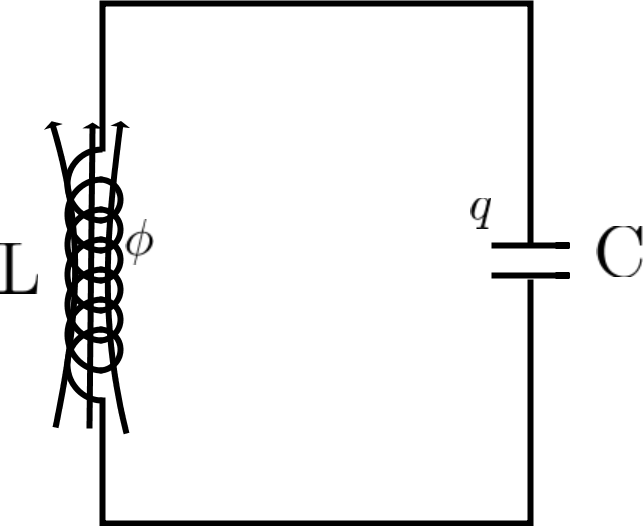
\includegraphics[width=150pt]{Figures/LC_oscillator}
\decoRule
\caption[LC oscillator]{LC oscillator circuit}
\label{fig:LC oscillator}
\end{figure}

The LC oscillator, shown in Fig.\ref{fig:LC oscillator}, when treated classically has a charge $q$ on the capacitor, and a flux $\phi$ in the inductor. The flux is related to the charge via the inductance as $\phi=L\dfrac{dq}{dt}$. The Hamiltonian for this circuit is
\begin{equation}
\mathcal{H}=\frac{q^2}{2C}+\frac{\phi^2}{2L}
\end{equation}

\subsubsection{Quantum LC oscillator}

Observe that the 2 variables involved in the LC oscillator, $q$ and $\phi=L\dfrac{dq}{dt}$, are similar in form to the position and momentum operators in quantum mechanics, $\hat{x}$ and $\hat{p}=-j\hbar\dfrac{\partial}{\partial x}$. Even the Hamiltonian is of the same form.\parencite{Devoret1995}
\begin{equation}
\hat{\mathcal{H}}=\frac{\hat{p}^2}{2m}+\frac{m\omega^2\hat{x}^2}{2}
\end{equation}
Because of this, we can treat this circuit like the simple harmonic oscillator and introduce the annihilation and creation operators to define $\hat{q}$, $\hat{\phi}$ and Hamiltonian operators as
\begin{subequations}
\begin{align}
\hat{q}&=\frac{1}{j}\sqrt{\frac{\hbar}{2Z_0}}(a-a^\dag)\\
\hat{\phi}&=\sqrt{\frac{\hbar Z_0}{2}}(a+a^\dag)\\
\hat{\mathcal{H}}&=\frac{\hbar\omega_0}{2}(a^\dag a+aa^\dag)=\hbar\omega_0\left(a^\dag a + \frac{1}{2}\right)
\end{align}
\end{subequations}
where
\begin{align*}
[\hat{\phi},\hat{q}]=j\hbar&&
\omega_0=\frac{1}{\sqrt{LC}}&&
Z_0=\sqrt{\frac{L}{C}}
\end{align*}
$\omega_0$ and $C$ in the LC oscillator is analogous to $\omega$ and $m$ in the harmonic oscillator.

We can write the wave-functions of the energy eigenstates of the LC oscillator as
\begin{equation}
\bra{x}\ket{0}=\psi_0=\left(\frac{C\omega_0}{\pi\hbar}\right)^\frac{1}{4}e^{-\left(\frac{C\omega_0}{2\hbar}\right)x^2}
\end{equation}
This solution can be obtained using $a^\dag\ket{0}=0$

The rest of the eigenstates can be obtained by using the ladder operator $a$ since
\begin{equation}
a\ket{n}=\sqrt{n+1}\ket{n+1}
\end{equation}
which gives
\begin{equation}
\ket{n}=\frac{(a)^n}{\sqrt{n!}}\ket{0}
\end{equation}
The energy corresponding to these states are
\begin{equation}
E_n=\left(n+\frac{1}{2}\right)\hbar\omega_0
\end{equation}
The general solution to the Schr\"{o}dinger equation $\hat{\mathcal{H}}\ket{\psi}=E\ket{\psi}$ is
\begin{equation}
\ket{\psi}=\sum_nc_n\ket{n}
\end{equation}
The first few energy levels along with the corresponding wavefunctions are shown in Fig.\ref{fig:harmonic oscillator}.

\begin{figure}
\centering
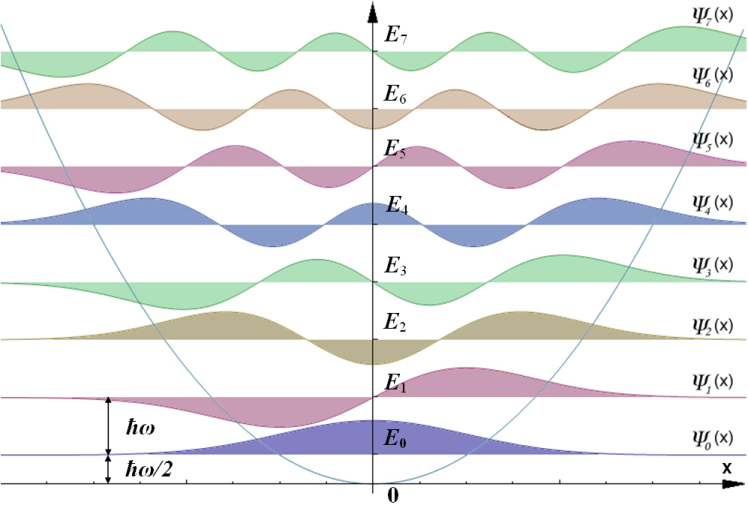
\includegraphics[width=\linewidth]{Figures/harmonic_oscillator}
\decoRule
\caption[Harmonic Oscillator Energy Levels]{The harmonic oscillator potential showing the Energy Levels $E_1,E_2,\ldots$ along with the corresponding wavefunctions $\psi_1,\psi_2,\ldots$. Replacing the position coordinate here with charge would give us the Energy levels for an LC oscillator.Taken from \\© \href{https://pl.wikipedia.org/wiki/Wikipedysta:Tomasz59}{User:Tomasz59} / \href{http://commons.wikimedia.org/}{Wikimedia Commons} / \href{http://creativecommons.org/licenses/by-sa/3.0/}{CC-BY-SA-3.0}}
\label{fig:harmonic oscillator}
\end{figure}

\subsubsection{Nonlinear Harmonic Oscillator}

Note that the energy levels in the Simple Harmonic Oscillator (SHO) or the LC oscillator are equispaced. This means that if we supply a photon of energy $\hbar\omega_0$ to the LC oscillator, we can change the state from any $\ket{n}$ to $\ket{n+1}$, and all photons emitted due to the transition from $\ket{n}$ to $\ket{n-1}$ will have the same energy.

A Nonlinear Harmonic Oscillator is one where the energy levels do not increase linearly. We can create a nonlinear oscillator by adding a perturbation to the Hamiltonian. The new Hamiltonian will be of the form
\begin{equation}
\hat{\mathcal{H}}=\frac{q^2}{2C}+\frac{\phi^2}{2L} +\mathcal{H}'
\end{equation}
where $H'$ is the perturbation term.
The energy levels for this new Hamiltonian can be written in terms of the unperturbed Hamiltonian using perturbation theory as
\begin{equation}
E_n=E_n^{(0)}+\expval{\mathcal{H}'}{n^{(0)}}+\sum_{k\neq n}\frac{\left|\mel{k^{(0)}}{\mathcal{H}'}{n^{(0)}}\right|^2}{E_n^{(0)}-E_k^{(0)}}+\ldots
\end{equation}
where,\\
$E_n$ is the new energy for the $n$th eigenstate,\\
$E_n^{(0)}$ is the energy for the $n$th eigenstate of the unperturbed Hamiltonian,\\
$\expval{\mathcal{H}'}{n^{(0)}}$ is the first order correction to the energy and\\
$\sum_{k\neq n}\frac{\left|\mel{k^{(0)}}{\mathcal{H}'}{n^{(0)}}\right|^2}{E_n^{(0)}-E_k^{(0)}}$ is the second order correction to the energy.

If the perturbation $\mathcal{H}'$ is not a constant (i.e $\mathcal{H}'(n)\neq \mathcal{H}'(m)$ where $n\neq m$), then we can access only the ground state and the first exited state with one frequency of photons. This is because if the particle is in the first excited state, and another photon of the same energy ($E_{10}=E_1-E_0$) is supplied to the system, it will not excite the particle further.

This means that we can selectively access only 2 states. If we can manipulate such a 2 level system and it's interactions, we have a qubit!

\subsection{The Josephson Junction}

The \JJ is the nonlinear element used in the described experiments due to it's negligible dissipation rate which is essential for working in the quantum regime.\\
The \JJ is made of 2 superconductors coupled by a weak link. In our case the junction is an S-I-S (Superconductor-Insulator-Superconductor) junction as shown in Fig.\ref{fig:SISJJ}.

\begin{figure}
\centering
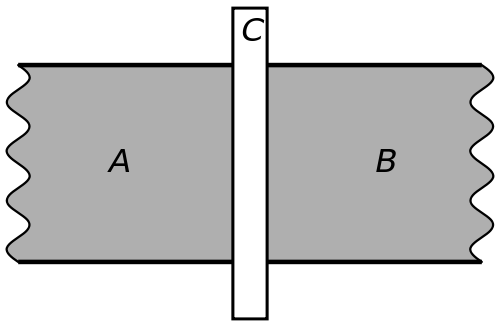
\includegraphics[width=\linewidth]{Figures/SISJJ}
\decoRule
\caption[Josephson Junction]{Simple geometric structure of a \JJ with A and B being superconducting regions and C being the thin insulating layer.}
\label{fig:SISJJ}
\end{figure}

Electrons in a normal metal behave like fermions. But at very low temperatures, they form cooper pairs that act like bosons. Nearly all the bosons will be at the lowest energy in exactly the same state \cite{Feynman1966}. This means that the superconductor will have a macroscopic wavefunction with a single homogeneous amplitude and phase.

In the \JJ, there are two superconductors, and so we can define 2 amplitudes and 2 phases corresponding to each superconductor.
\begin{align*}
\psi_1&=\sqrt{\rho_1}e^{j\theta_1}\\
\psi_2&=\sqrt{\rho_2}e^{j\theta_2}
\end{align*}
Then, the current and voltage characteristics are given by \cite{Harmans1997}
\begin{align}
I_s&=I_0\sin\delta
\label{eqn:JJ current}\\
V&=\frac{\Phi_0}{2\pi}\dot{\delta}
\label{eqn:JJ voltage}
\end{align}
where $\delta=\theta_2-\theta_1$ is the superconducting phase difference\footnote{This phase difference $\delta$ is the generalized phase difference $\delta=\Delta\theta-\displaystyle\dfrac{2\pi}{\Phi_0}\int A\cdot dl$} associated with the \JJ, $\Phi_0=h/2e$ is the flux quantum for a cooper pair and $I_0$ is the critical current of the junction.

We can view the \JJ as a nonlinear inductor and find the inductance simply by using $V=L_J\dfrac{dI_s}{dt}$ which gives $L_J$, the Josephson Inductance to be
\begin{equation}
L_J=\frac{\Phi_0}{2\pi}\frac{1}{I_0\cos\delta}
\end{equation}

In addition to this we can represent a real \JJ using the RCSJ model with a shunting capacitance ($C$) and resistance ($R$) along with the bare \JJ \cite{Harmans1997}. Then the current through the circuit is
\begin{equation}
I=I_s+\frac{V}{R}+C\frac{dV}{dt}
\end{equation}
by using \ref{eqn:JJ current} and \ref{eqn:JJ voltage} we get
\begin{equation}
C\left(\frac{\hbar}{2e}\right)^2\frac{d^2\delta}{dt^2}+\frac{1}{R}\left(\frac{\hbar}{2e}\right)^2\frac{d\delta}{dt}+\frac{\hbar}{2e}(I_0\sin\delta-I)=0
\end{equation}
We can see that this is the equation of motion of a particle moving along the $\delta$ coordinate with\\ an acceleration $\dfrac{d^2\delta}{dt^2}$,\\ drag force proportional to velocity $\dfrac{d\delta}{dt}$ and\\ force due to the gradient of the potential energy as the last term.\\
This leads to the "particle mass" given by
\begin{align}
M&=C\left(\frac{\hbar}{2e}\right)^2&&\text{"particle mass"}\\
U(I,\delta)&=-E_J\cos\delta-\left(\frac{\hbar}{2e}\right)I\delta&&\text{potential energy}
\end{align}
where $E_J$, the Josephson Energy is given by
\begin{equation}
E_J=\frac{\hbar}{2e}I_0=\frac{\Phi_0}{2\pi}I_0
\end{equation}
The current $I$ is usually so small that we can ignore that term making the potential energy
\begin{equation}
U=-E_J\cos\delta
\label{eqn:JJ potential energy}
\end{equation}

The electrical energy stored in the capacitance is analogous to kinetic energy and can be calculated as
\begin{equation}
E_{kin}=\frac{1}{2}Mv^2=\frac{1}{2}C\left(\frac{\hbar}{2e}\right)^2\left(\frac{d\delta}{dt}\right)^2
\end{equation}

\subsection{The Cooper Pair Box}

The \CPB circuit is shown in Fig.\ref{fig:cooperpairbox}. It consists of a superconducting island capacitively coupled (with capacitance $C_g$) to a voltage source ($V_g$) connected to ground, and a \JJ connected to the ground. The \JJ can be represented by a capacitance ($C_j$) and the bare \JJ (represented by $E_j$) as shown in the figure.

\begin{figure}
\centering
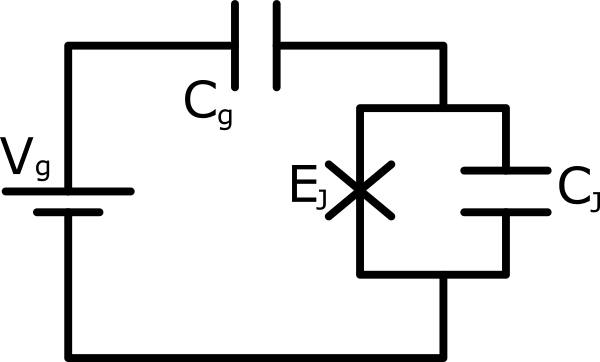
\includegraphics{Figures/CPB}
\decoRule
\caption[\CPB circuit]{The \CPB circuit with the \JJ represented as a bare \JJ with Josephson Energy $E_J$ and a capacitance $C_j$.}
\label{fig:cooperpairbox}
\end{figure}

The electrical energy of this circuit is the energy stored in the 2 capacitors, $C_g$ and $C_j$. If the total charge of the superconducting island is $-n|e|$, then the electrical energy ($\mathcal{H}_{el}$) is given by \cite{Schuster2007}
%---------------------------------------------------------
% Maybe you can show this in Appendix
%--------------------------------------------------------
\begin{equation}
\hat{\mathcal{H}_{el}}=4E_C(\hat{n}-n_g)^2
\end{equation}
where $\hat{n}\ket{n}=n\ket{n}$, $\ket{n}$ is the charge state with $n$ cooper pairs.\\
$E_C=e^2/2C_\Sigma=e^2/2(Cj+Cg)$ is the energy required to add one electron to the island and $n_g=C_gV_g/e$.\\
The energy levels are shown in Fig.\ref{fig:CPB EJ=0} for $E_J=0$. The \JJ would allow charge to tunnel through at $n_g=0.5,-0.5,1.5,-1.5\ldots$ in order to maintain the lowest energy.

%---------E_J=0 energy levels---------------------------

However, to calculate the complete Hamiltonian, we must also take into account the energy of the bare \JJ ($H_J$) which is given by.
\begin{equation}
\hat{\mathcal{H}_J}=-E_J\cos\hat{\delta}
\end{equation}
This is the tunnelling energy in the phase basis. To find the expression in the charge basis, we start with the commutation relation between charge and phase (See Appendix 1-A-2 from \cite{Cottet2002d}).
\begin{align}
\left[\hat{n},\hat{\delta}\right]&=-j
\end{align}
Using this and the commutator identity \ref{eqn:comm identity}, we get \ref{eqn:n->n+p}.
\begin{align}
\left[\hat{n},\hat{\delta}^m\right]&=\hat{\delta}^{m-1}\left[\hat{n},\hat{\delta}\right]+\hat{\delta}\left[\hat{n},\hat{\delta}^{m-1}\right]
\label{eqn:comm identity}\\
\end{align}
we can recursively use this relation to get
\begin{align}
\left[\hat{n},\hat{\delta}^m\right]&=-jm(\hat{\delta})^{m-1}\\
\hat{n}\hat{\delta}^m&=-jm\hat{\delta}^{m-1}+\hat{\delta}^m\hat{n}
\end{align}
The operator $\hat{n}e^{jp\hat{\delta}}$ after expansion is
\begin{align}
\begin{split}
\hat{n}e^{jp\hat{\delta}}&=\hat{n}\sum_{m=0}^\infty \frac{( jp\hat{\delta})^m}{m!}=\sum_{m=0}^\infty \frac{(jp)^m\hat{n}\hat{\delta}^m}{m!}\\
&=\sum_{m=0}^\infty \frac{(jp)^m\hat{n}(\hat{\delta})^m}{m!}\\
&=\sum_{m=0}^\infty \frac{(jp)^m(-jm\hat{\delta}^{m-1}+\hat{\delta}^m\hat{n})}{m!}\\
&=\sum_{m=0}^\infty \frac{(jp)^m(-jm\hat{\delta}^{m-1})}{m!}+\sum_{m=0}^\infty \frac{(jp\hat{\delta})^m\hat{n}}{m!}\\
&=p\sum_{m=1}^\infty \frac{(jp\hat{\delta})^{m-1}}{(m-1)!}+\sum_{m=0}^\infty \frac{(jp\hat{\delta})^m\hat{n}}{m!}
\end{split}\\
\hat{n}e^{jp\hat{\delta}}&=pe^{jp\hat{\delta}}+e^{jp\hat{\delta}}\hat{n}
\end{align}
Using this operator on the charge state $\ket{n}$ gives
\begin{align}
\hat{n}\lbrace e^{jp\hat{\delta}}\ket{n}\rbrace&=pe^{jp\hat{\delta}}\ket{n}+e^{jp\hat{\delta}}\hat{n}\ket{n}\\
&=(n+p)\lbrace e^{jp\hat{\delta}}\ket{n}\rbrace\\
\implies e^{jp\hat{\delta}}\ket{n}&=\ket{n+p}
\end{align}
So, we can see that
\begin{align}
e^{ip\hat{\delta}}&=\sum_{m=-\infty}^\infty \ket{m+p}\bra{m}\\
\begin{split}
\cos\hat{\delta}=\frac{1}{2}\left(e^{i\hat{\delta}}+e^{-i\hat{\delta}}\right)&=\frac{1}{2}\left(\sum_{m=-\infty}^\infty \ket{m+1}\bra{m}+\sum_{m=-\infty}^\infty \ket{m-1}\bra{m}\right)\\
&=\frac{1}{2}\sum_{n=-\infty}^{+\infty}\ket{n}\bra{n+1}+\ket{n+1}\bra{n}
\end{split}
\end{align}
\begin{equation}
\hat{\mathcal{H}_J}=-\frac{E_J}{2}\left(\sum_{n=-\infty}^{+\infty}\ket{n}\bra{n+1}+\ket{n+1}\bra{n}\right)
\end{equation} 

So the complete Hamiltonian in the charge basis is the sum of these
\begin{equation}
\hat{\mathcal{H}}=\sum_{n=-\infty}^{+\infty}\left(4E_C(\hat{n}-n_g)^2\ket{n}\bra{n}-\frac{E_J}{2}\ket{n}\bra{n+1}+\ket{n+1}\bra{n}\right)
\end{equation}

In the phase basis we can replace $\hat{n}$ with $-i\dfrac{\partial}{\partial\delta}$ to get
\begin{equation}
\hat{\mathcal{H}}=4E_C\left(-i\frac{\partial}{\partial\delta}-n_g\right)^2-E_J\cos\delta
\end{equation}

The energy eigenstates $\ket{k}$ are given by the schr\"{o}dinger equation
\begin{equation}
\hat{\mathcal{H}}(n_g)\ket{k}=E_k\ket{k}
\end{equation}

The energy levels ($E_k$) plotted against gate charge ($n_g$) for different $E_J/E_C$ values are shown in Fig.\ref{fig:diff EJ/EC}.

%-----------Fig for different EJ/EC---------------------

As we can see the charge noise is very low for the case of high $E_J/E_C$. Also, anharmonicity, which is defined as $\alpha=E_{21}-E_{10}$, is reduced but not zero. In-fact, charge noise reduces exponentially while anharmonicity reduces only algebraically as $E_J/E_C$ is increased. This is the basis on which the transmon qubit is realised.

\subsection{The 3D Superconducting Transmon}

A Transmon is basically a \CPB in which the \JJ is shunted with a large capacitance in order to decrease $E_C$ and so increase $E_J/E_C$.